\documentclass[blind]{sig-alternate-05-2015}
\usepackage{flushend}
\usepackage{graphicx}
%\usepackage[justification=centering]{caption}
\usepackage{algorithm}
\usepackage{algorithmic}
\usepackage{multirow}
\usepackage{amsmath}
\usepackage{xcolor}
\usepackage{colortbl}
\usepackage{cite}
\usepackage{listings}
\usepackage[square, comma, sort&compress, numbers]{natbib}
\usepackage{verbatim}
\DeclareMathOperator*{\argmin}{argmin}

 
\linespread{0.9625}


\clubpenalty = 10000
\widowpenalty = 10000
\displaywidowpenalty = 10000


\newcommand{\commentout}[1]{ }



 \newcommand{\superscript}[1]{\ensuremath{^{\textrm{#1}}}}

 \def\sharedaffiliation{\end{tabular}\newline\begin{tabular}{c}}
 
 \def\wu{\superscript{*}}
 \def\wg{\superscript{\dag}}
 \def\wdg{\superscript{\ddag}}

\lstset{ %
  language=c,
	backgroundcolor=\color{white},   % choose the background color; you must add \usepackage{color} or \usepackage{xcolor}
	basicstyle=\scriptsize\ttfamily,  % the size of the fonts that are used for the code
	breakatwhitespace=false,         % sets if automatic breaks should only happen at whitespace
	breaklines=true,                 % sets automatic line breaking
	captionpos=b,                    % sets the caption-position to bottom
	commentstyle=\color{mygreen},    % comment style
	deletekeywords={...},            % if you want to delete keywords from the given language
  escapeinside={(*}{*)},          % if you want to add LaTeX within your code
	extendedchars=true,              % lets you use non-ASCII characters; for 8-bits encodings only, does not work with UTF-8
	frame=single,                    % adds a frame around the code
	keepspaces=true,                 % keeps spaces in text, useful for keeping indentation of code (possibly needs columns=flexible)
	keywordstyle=\color{blue},       % keyword style
	morekeywords={*,...},            % if you want to add more keywords to the set
	numbers=none,                    % where to put the line-numbers; possible values are (none, left, right)
	numbersep=5pt,                   % how far the line-numbers are from the code
	numberstyle=\color{black},       % the style that is used for the line-numbers
	rulecolor=\color{black},         % if not set, the frame-color may be changed on line-breaks within not-black text (e.g. comments (green here))
	showspaces=false,                % show spaces everywhere adding particular underscores; it overrides 'showstringspaces'
	showstringspaces=false,          % underline spaces within strings only
	showtabs=false,                  % show tabs within strings adding particular underscores
	stepnumber=1,                    % the step between two line-numbers. If it's 1, each line will be numbered
	stringstyle=\color{mymauve},     % string literal style
	tabsize=2,                       % sets default tabsize to 2 spaces
	%title=\lstname,                   % show the filename of files included with \lstinputlisting; also try caption instead of title
%	linewidth=0.45\textwidth,
}




%%-----------remove copyright plate-------
\makeatletter
\def\@copyrightspace{\relax}
\makeatother
%%----------------------------------------

\begin{document}

% Copyright
\setcopyright{acmcopyright}
%\setcopyright{acmlicensed}
%\setcopyright{rightsretained}
%\setcopyright{usgov}
%\setcopyright{usgovmixed}
%\setcopyright{cagov}
%\setcopyright{cagovmixed}


% DOI
%\doi{10.475/123_4}

% ISBN
%\isbn{123-4567-24-567/08/06}

%Conference
%\conferenceinfo{PLDI '13}{June 16--19, 2013, Seattle, WA, USA}

%\acmPrice{\$15.00}

%
% --- Author Metadata here ---
%\conferenceinfo{WOODSTOCK}{'97 El Paso, Texas USA}
%\CopyrightYear{2007} % Allows default copyright year (20XX) to be over-ridden - IF NEED BE.
%\crdata{0-12345-67-8/90/01}  % Allows default copyright data (0-89791-88-6/97/05) to be over-ridden - IF NEED BE.
% --- End of Author Metadata ---

\title{GUI Testing as a Service}


\maketitle

\begin{abstract}
  abstract
\end{abstract}

\section{Introduction}\label{section:introduction}

Graphic User Interface(GUI) applications are driven by user events.

Manually testing of GUI is labor intensive.

\texttt{Guitar} \cite{guitar} uses an automatic method to test GUI. It automatically generate event sequences for java GUI applications. But it use built-in concrete value for user inputs. Although it also accepts alternative user inputs, however itself doesn't provide any facility to generate user inputs.

\texttt{Barad} \cite{barad} is a novel GUI testing framework based on symbolic execution. It can obtain data inputs through executing symbolically test cases which are chains of event listener method invocations. It manually created symbolic mirror of java GUI library, so its released source code contains a large symbolic java GUI library. however it lacks necessary documentation, it is very hard to deploy the project, and such a heavy code base might be hard to maintain or error pruning.

\texttt{jfp-awt} \cite{jpfawt} is an extension of the Java PathFinder for java GUI application model checking. It needs the user to specify sets of interaction sequences, for a real GUI application, this might be labor intensive task for testers.

In the paper we present a novel tool \texttt{Guicat} which generate concrete user inputs to cover different program branch. We build our work on top of \texttt{Guitar} and \texttt{Catg} \cite{catg}.




\section{Motivating Example}

\begin{figure}
\label{fig:ex}
  \centering
  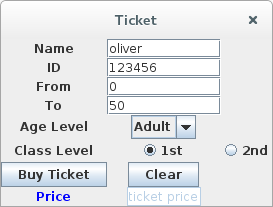
\includegraphics[width=50mm,scale=0.5]{./res/ticket.png}
  \caption{GUI for train ticket purchase}
\end{figure}

The GUI shown in Figure~\ref{fig:ex} is an application that we developed to mimic the motivating example used in Barad~\cite{}. calculate the price for a train ticket. The application calculates the price for a train ticket based on the information passed through the GUI. A user must provide a passenger class, name, ID, age level, and begin
and end points. Each passenger class has its own coefficient that is used during the calculation. Each age level has a different
base price depending on the distance to be traveled,
which is the difference between From mile and To mile. Figure~\ref{fig:code} gives the code snippet of the calculation logic.  There are twenty two branches with conditional statements nested three levels deep. The
execution of a particular branch depends on the user
input both in the form of data and event sequence (i.e.
selecting a radio button).


This program is used to calculate ticket price according to different properties of the client, such as the class level, or age, or the travel distance. When the \texttt{Buy} button is clicked, the application check the \texttt{Name} and \texttt{ID} input, if the length of the \texttt{Name} string is less or equal than 3, or \texttt{ID} equals to some special string, then the application will display an error message and will not calculate any price. After checking the user information successfully, the application start to calculate the price as follows: read the user class input and set a coefficient for the price, read the user age to go to different pricing branch, read the start and dest input and calculate the distance of travelling, then calculate the price. We can see from the following code snippets that there should be many branches in the code to calculate ticket price for all kinds of clients.
\begin{figure}
\label{fig:code}
\begin{lstlisting}
  int maxPrice = 100;
  int minPrice = 10;
  int coefficient = (classLevel == TicketModel.FIRSTCLASS) ? 2 : 1;
  int dist = to - from;
  if (ageLevel == Adult) {
    if (dist < 40) {
      price = 100 * coeficient;
    } else if (dist < 45) {
      price = 110 * coeficient;
    } else if (dist < 50) {
      price = 120 * coeficient;
    } else if (dist < 70) {
      price = 140 * coeficient;
    } else if (dist < 80) {
      price = 150 * coeficient;
    } else if (dist < 85) {
      price = 155 * coeficient;
    } else if (dist < 100) {
      price = 160 * coeficient;
    }
  }
  assert(price<=maxPrice&&price>=minPrice);
\end{lstlisting}
\caption{Code snippet for calculating ticket price}
\end{figure}

One can not claim this kind of applications are well tested until all the branches has been covered during test stage.

\section{Algorithms}

\begin{algorithm}[htbp]
\caption{TestGeneration(program $GUI$, int $B$, int $S$)}
\label{alg:top}
\begin{algorithmic}[1]
\STATE SET chains = $N_0$.ProduceEventSequence($B$); 
%\STATE SET chains = $N_0$.ChainReduction(chains);
\FORALL {$c \in chains$}
	\STATE $N_i$ = AllocateTask();
	\STATE tests.add($N_i$.SymbolicExecution(c));
\ENDFOR
\end{algorithmic}
\end{algorithm}

\section{Implementation}

\subsection{Architecture}

The architecture is described as Figure ~\ref{figure:architecture}

\begin{figure}
  \centering
  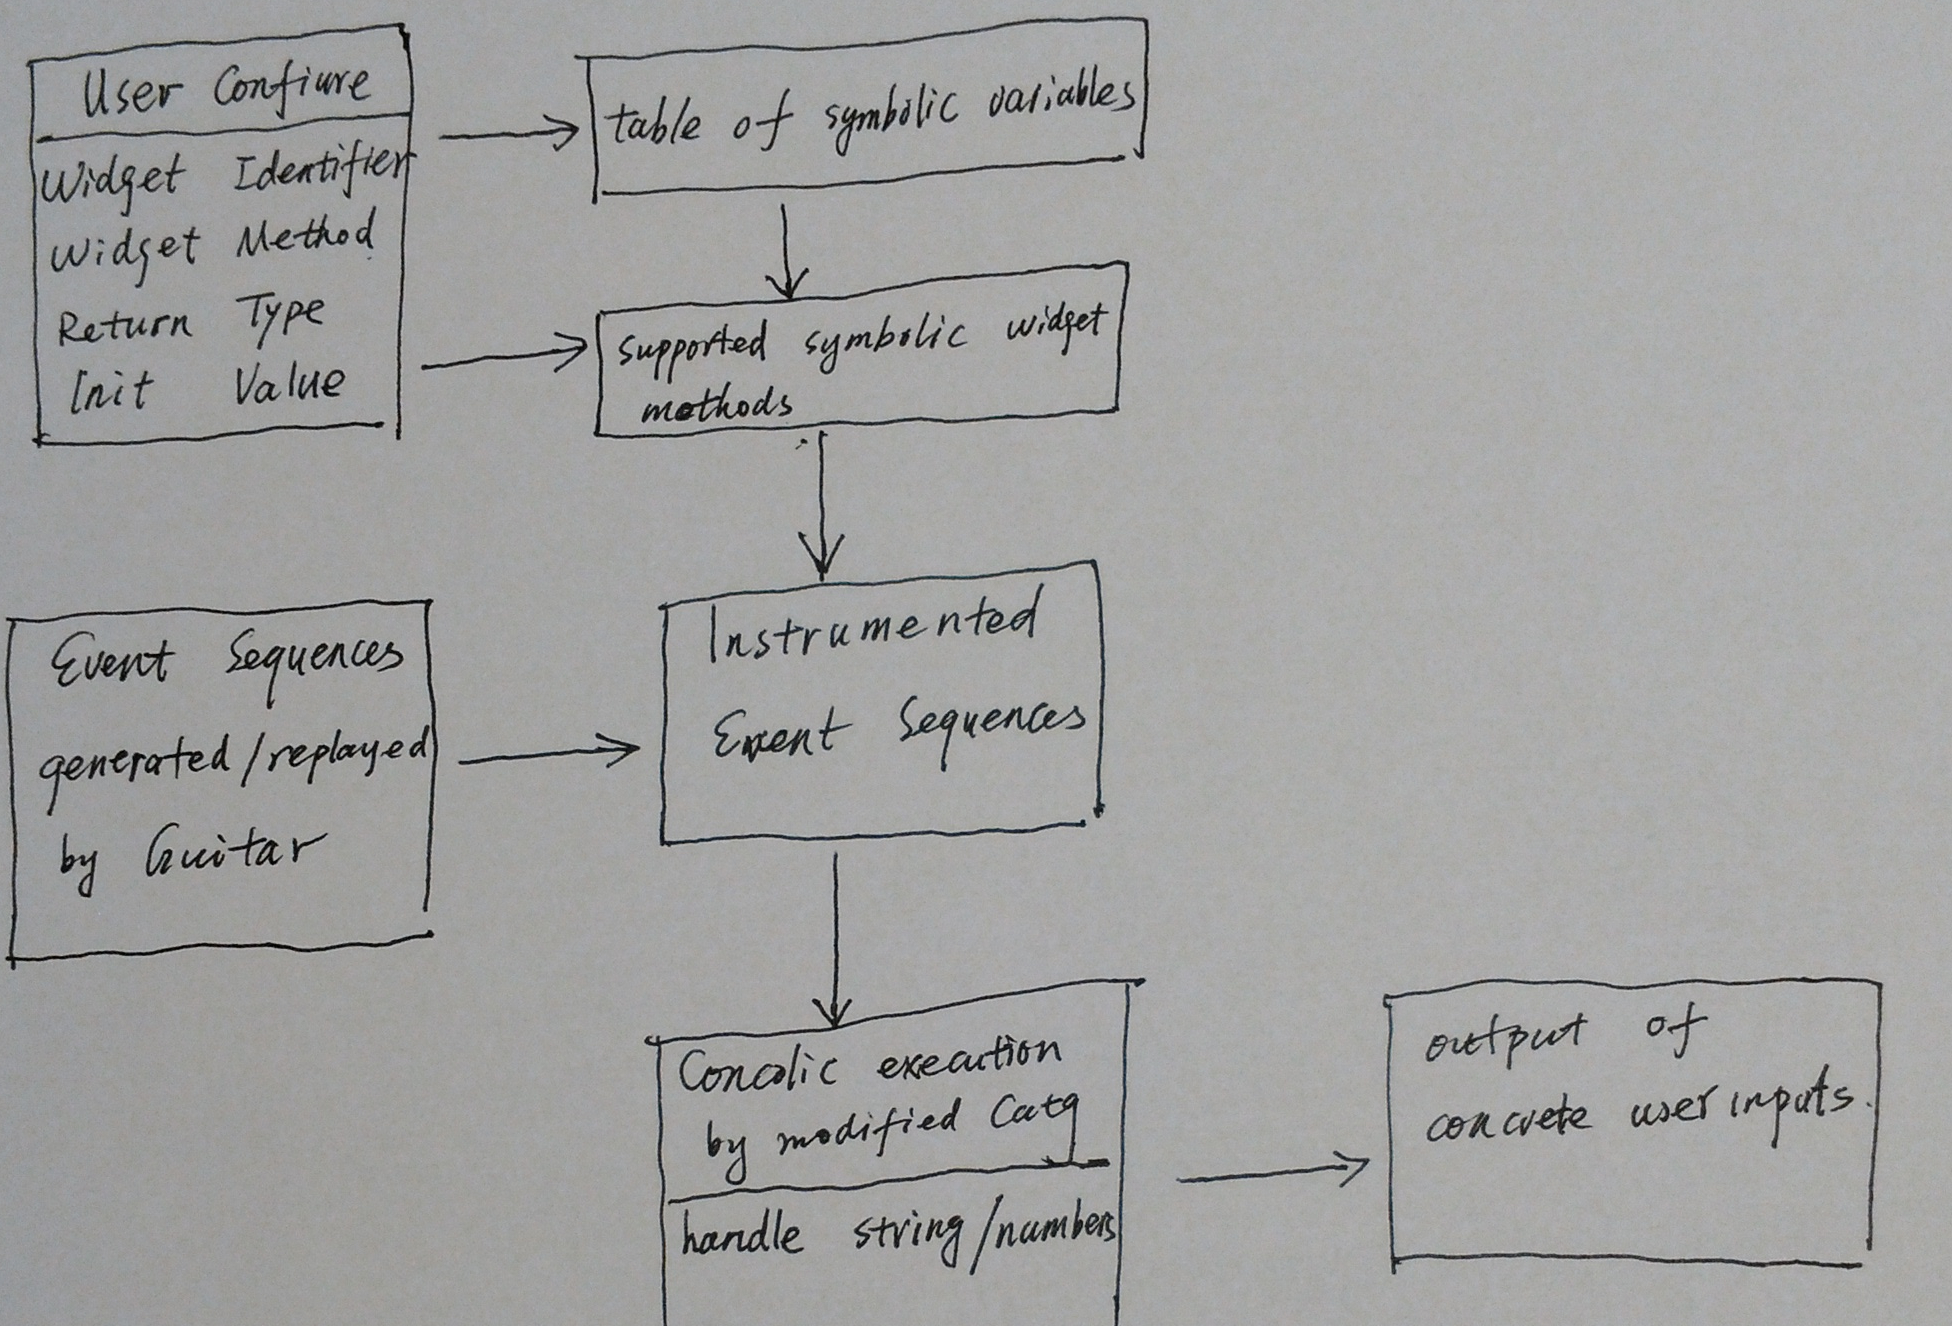
\includegraphics[width=100mm,scale=0.5]{./res/archi-hand.jpg}
  \caption{architecture}
  \label{figure:architecture}
\end{figure}

Our goal is to generate user inputs for java GUI applications to achieve high branch and code coverage.

The \textbf{work-flow} is  we let the tester to create a configuration file, indicating which variables should be symbolic.
Based on the configure file we create symbolic variables and symbolic functions which are used to replace the corresponding one in the \textbf{replayed sequences}. We generate replayed sequenses from guitar. Using guitar replayer to replay one event sequence is a replayed sequence. We do the replacement by \texttt{javaagent} using \texttt{ASM} the same way as \texttt{CATG} does. After replacement, we get an instrumented replayed sequence, then we can sent it to catg to do concolic execution. we use shell scripts to glue up modules for the testing process of an AUT.

We handle the problem that for a number input, java GUI framework returns a String to programmer by built in function \textit{getText()}, and the programmer somewhere parse the String to numbers using \textit{Integer.parseInt} or something similar.  Because \texttt{CATG} can't handle this kind of operation, we modify catg to support casting functions like \textit{Integer.parseInt}.

Note that catg requires the tester to set up symbolic variables in source code, and this may be inconvenient when source code is not available. We have automated this process.

The following are details of different modules
\begin{itemize}
  \item{\textbf{configuration file} contains entries of symbolic variable information. Each entry contains four elements separated by comma: widget identifier, widget method, return type, init value. A widget identifier is the \textit{accessibleName} of the java widget, it is set by \textit{setAccessibleName} or \textit{setLabelFor}. Jpf-awt uses the same identifier. (Not certain whether guitar uses the same one or not)}. A widget method is the method which should be replaced by a symbolic one. It is usually a built in function which is used to get user input like \textit{getText, isSelected, getActionCommand}. A return type is the type of this symbolic variable. A feasible return type should be one value in this list: {String,int, long, char, byte, short, boolean}. A init value is the concrete value of the symbolic variable for the symbolic execution to start with.

  \item{\textbf{table of symbolic variables}} is a set of symbolic variables created using the configuration file. It is stored in a \textit{LinkedListedMap} to keep the order of the variables. For each entry in the configuration file, we create exactly one entry in the map whose key is the widget identifier, value is an symbolic entry object. If the return type is String, the symbolic entry object contains a symbolic string variable, if the return type is something else like an int, the symbolic entry object contains a symbolic string variable and a symbolic int variable. To the tester, the symbolic int variable is hidden, the output will write back to the String variable.

  \item{\textbf{supported symbolic functions}} is a collection of manually created functions which are used to replace the corresponding ones in the replayed sequences. For example, we create a static function \textit{SGetText(Object)} for the \textit{getText()} of \textit{javax.swing.TextInput}. A little trick here is to pass the object  to the static function parameter so that the stack frames don't need change.

  \item{\textbf{instrumentation} We use ASM to instrument java bytecode. We replace the function call with a symbolic one if it satisfies the following conditions: 1. the call is from an object which has an widget identifier exists in the configuration file; 2. the function name exists in the configuration file}

    \item{\textbf{parseInt support}}. We add parseInt support to catg. When the symbolic string is transformed to int by \textit{parseInt}, catg doesn't support this function originally, so falls to concrete execution. We modify catg to add this support. When the catg encounters \textit{parseInt}, we check the string. if the string is one in the symbolic table, and there is an int symbolic variable in the same symbolic entry, we use this int symbolic value as the return value of  catg's symbolic call \textit{parseInt}, so catg can continue execute symbolically. We have modified 3 files in catg's originmal source.

\end{itemize}


\section{experiment}
We have tested ticket seller. We user guitar to generate testcase. Each guitar test case we have get up to 13 concrete inputs.

if we set guitar event sequences length to 1, then guitar will genenrate 10 testcases, we can generate 82 testcases.
if we set guitar event sequences length to 2, then guitar will genenrate 89 testcases, we can generate 952 testcases.


\bibliographystyle{unsrt}
\bibliography{paper}




\end{document}
